%%%%%%%%%%%%%%%%%%%%%%%%%%%%%%%%%%%%%%%%%
% Programming/Coding Assignment
% LaTeX Template
%
% This template has been downloaded from:
% http://www.latextemplates.com
%
% Original author:
% Ted Pavlic (http://www.tedpavlic.com)
%
% Note:
% The \lipsum[#] commands throughout this template generate dummy text
% to fill the template out. These commands should all be removed when 
% writing assignment content.
%
% This template uses a Perl script as an example snippet of code, most other
% languages are also usable. Configure them in the "CODE INCLUSION 
% CONFIGURATION" section.
%
%%%%%%%%%%%%%%%%%%%%%%%%%%%%%%%%%%%%%%%%%

%----------------------------------------------------------------------------------------
%	PACKAGES AND OTHER DOCUMENT CONFIGURATIONS
%----------------------------------------------------------------------------------------

\documentclass{article}

\usepackage{fancyhdr} % Required for custom headers
\usepackage{lastpage} % Required to determine the last page for the footer
\usepackage{extramarks} % Required for headers and footers
\usepackage[usenames,dvipsnames]{color} % Required for custom colors
\usepackage{graphicx} % Required to insert images
\usepackage{listings} % Required for insertion of code
\usepackage{courier} % Required for the courier font
\usepackage{lipsum} % Used for inserting dummy 'Lorem ipsum' text into the template

% Margins
\topmargin=-0.45in
\evensidemargin=0in
\oddsidemargin=0in
\textwidth=6.5in
\textheight=9.0in
\headsep=0.25in

\linespread{1.1} % Line spacing

% Set up the header and footer
\pagestyle{fancy}
\lhead{\hmwkAuthorName} % Top left header
\chead{\hmwkClass\ (\hmwkClassInstructor\ \hmwkClassTime): \hmwkTitle} % Top center head
\rhead{\firstxmark} % Top right header
\lfoot{\lastxmark} % Bottom left footer
\cfoot{} % Bottom center footer
\rfoot{Page\ \thepage\ of\ \protect\pageref{LastPage}} % Bottom right footer
\renewcommand\headrulewidth{0.4pt} % Size of the header rule
\renewcommand\footrulewidth{0.4pt} % Size of the footer rule

\setlength\parindent{0pt} % Removes all indentation from paragraphs

%----------------------------------------------------------------------------------------
%	CODE INCLUSION CONFIGURATION
%----------------------------------------------------------------------------------------

\definecolor{MyDarkGreen}{rgb}{0.0,0.4,0.0} % This is the color used for comments
\lstloadlanguages{Perl} % Load Perl syntax for listings, for a list of other languages supported see: ftp://ftp.tex.ac.uk/tex-archive/macros/latex/contrib/listings/listings.pdf
\lstset{language=Perl, % Use Perl in this example
        frame=single, % Single frame around code
        basicstyle=\small\ttfamily, % Use small true type font
        keywordstyle=[1]\color{Blue}\bf, % Perl functions bold and blue
        keywordstyle=[2]\color{Purple}, % Perl function arguments purple
        keywordstyle=[3]\color{Blue}\underbar, % Custom functions underlined and blue
        identifierstyle=, % Nothing special about identifiers                                         
        commentstyle=\usefont{T1}{pcr}{m}{sl}\color{MyDarkGreen}\small, % Comments small dark green courier font
        stringstyle=\color{Purple}, % Strings are purple
        showstringspaces=false, % Don't put marks in string spaces
        tabsize=5, % 5 spaces per tab
        %
        % Put standard Perl functions not included in the default language here
        morekeywords={rand},
        %
        % Put Perl function parameters here
        morekeywords=[2]{on, off, interp},
        %
        % Put user defined functions here
        morekeywords=[3]{test},
       	%
        morecomment=[l][\color{Blue}]{...}, % Line continuation (...) like blue comment
        numbers=left, % Line numbers on left
        firstnumber=1, % Line numbers start with line 1
        numberstyle=\tiny\color{Blue}, % Line numbers are blue and small
        stepnumber=5 % Line numbers go in steps of 5
}

% Creates a new command to include a perl script, the first parameter is the filename of the script (without .pl), the second parameter is the caption
%\newcommand{\pythonscript}[2]{
%\begin{itemize}
%\item[]\lstinputlisting[caption=#2,label=#1]{#1.pl}
%\end{itemize}
%}

%----------------------------------------------------------------------------------------
%	DOCUMENT STRUCTURE COMMANDS
%	Skip this unless you know what you're doing
%----------------------------------------------------------------------------------------

% Header and footer for when a page split occurs within a problem environment
\newcommand{\enterProblemHeader}[1]{
\nobreak\extramarks{#1}{#1 continued on next page\ldots}\nobreak
\nobreak\extramarks{#1 (continued)}{#1 continued on next page\ldots}\nobreak
}

% Header and footer for when a page split occurs between problem environments
\newcommand{\exitProblemHeader}[1]{
\nobreak\extramarks{#1 (continued)}{#1 continued on next page\ldots}\nobreak
\nobreak\extramarks{#1}{}\nobreak
}

\setcounter{secnumdepth}{0} % Removes default section numbers
\newcounter{homeworkProblemCounter} % Creates a counter to keep track of the number of problems

\newcommand{\homeworkProblemName}{}
\newenvironment{homeworkProblem}[1][Problem \arabic{homeworkProblemCounter}]{ % Makes a new environment called homeworkProblem which takes 1 argument (custom name) but the default is "Problem #"
\stepcounter{homeworkProblemCounter} % Increase counter for number of problems
\renewcommand{\homeworkProblemName}{#1} % Assign \homeworkProblemName the name of the problem
\section{\homeworkProblemName} % Make a section in the document with the custom problem count
\enterProblemHeader{\homeworkProblemName} % Header and footer within the environment
}{
\exitProblemHeader{\homeworkProblemName} % Header and footer after the environment
}

\newcommand{\problemAnswer}[1]{ % Defines the problem answer command with the content as the only argument
\noindent\framebox[\columnwidth][c]{\begin{minipage}{0.98\columnwidth}#1\end{minipage}} % Makes the box around the problem answer and puts the content inside
}

\newcommand{\homeworkSectionName}{}
\newenvironment{homeworkSection}[1]{ % New environment for sections within homework problems, takes 1 argument - the name of the section
\renewcommand{\homeworkSectionName}{#1} % Assign \homeworkSectionName to the name of the section from the environment argument
\subsection{\homeworkSectionName} % Make a subsection with the custom name of the subsection
\enterProblemHeader{\homeworkProblemName\ [\homeworkSectionName]} % Header and footer within the environment
}{
\enterProblemHeader{\homeworkProblemName} % Header and footer after the environment
}

%----------------------------------------------------------------------------------------
%	NAME AND CLASS SECTION
%----------------------------------------------------------------------------------------

\newcommand{\hmwkTitle}{Assignment\ \#2} % Assignment title
\newcommand{\hmwkDueDate}{Thursday,\ September\ 25,\ 2014} % Due date
\newcommand{\hmwkClass}{CS\ 595} % Course/class
\newcommand{\hmwkClassTime}{4::20PM} % Class/lecture time
\newcommand{\hmwkClassInstructor}{Dr Nelson} % Teacher/lecturer
\newcommand{\hmwkAuthorName}{Victor Nwala} % Your name

%----------------------------------------------------------------------------------------
%	TITLE PAGE
%----------------------------------------------------------------------------------------

\title{
\vspace{2in}
\textmd{\textbf{\hmwkClass:\ \hmwkTitle}}\\
\normalsize\vspace{0.1in}\small{Due\ on\ \hmwkDueDate}\\
\vspace{0.1in}\large{\textit{\hmwkClassInstructor\ \hmwkClassTime}}
\vspace{3in}
}

\author{\textbf{\hmwkAuthorName}}
\date{} % Insert date here if you want it to appear below your name

%----------------------------------------------------------------------------------------

\begin{document}

\maketitle

%----------------------------------------------------------------------------------------
%	TABLE OF CONTENTS
%----------------------------------------------------------------------------------------

%\setcounter{tocdepth}{1} % Uncomment this line if you don't want subsections listed in the ToC

\newpage
\tableofcontents
\newpage

%----------------------------------------------------------------------------------------
%	PROBLEM 1
%----------------------------------------------------------------------------------------

% To have just one problem per page, simply put a \clearpage after each problem

\begin{homeworkProblem}
%Listing \ref{twitter.py} shows a Python script.
1.  Write a Python program that extracts 1000 unique links from
Twitter.
\lstinputlisting[breaklines=true, caption=twitter.py]{twitter.py}
This script extracts random urls from twitter related to the topic inside the filter at the end of the code.
I used several filters such as music, movies, football. The UrIs extracted may be duplicates or even nonexistent. I wrote
two other scripts to correct this. 
\begin{figure}
    \centering
    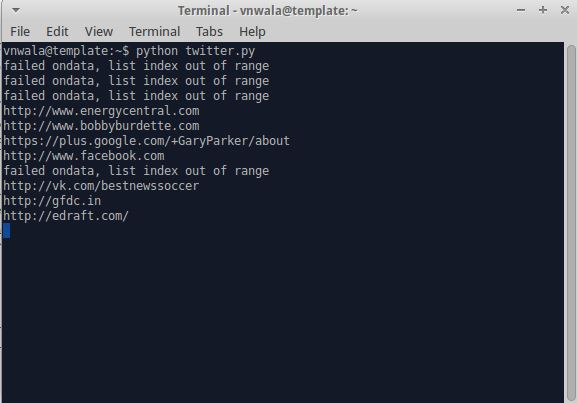
\includegraphics[width=3.0in]{TwitterUri}
    \caption{Screen Shot of twitter.py at work}
    \label{fig:1}
\end{figure}


%Listing \ref{preProcess.py} shows a Python script.

\lstinputlisting[breaklines=true, caption=preProcess.py]{preProcess.py}
\begin{figure}
    \centering
    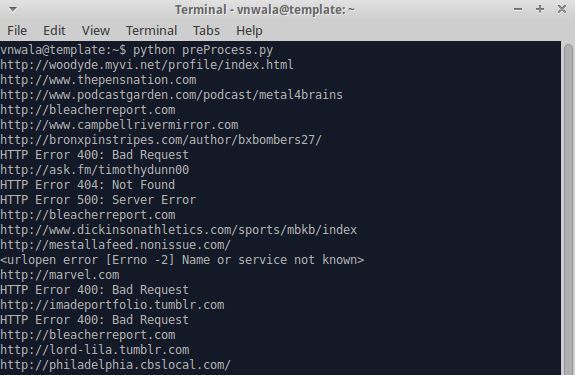
\includegraphics[width=3.0in]{preProcess}
    \caption{Screen Shot of preProcess.py at work}
    \label{fig:2}
\end{figure}
\begin{figure}
    \centering
    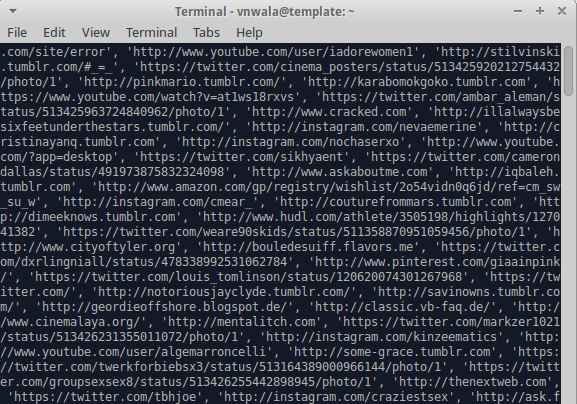
\includegraphics[width=3.0in]{processed}
    \caption{Screen Shot of processed.py at work}
    \label{fig:3}
\end{figure}
%\pythonscript{preProcess.py}{Python Script to extract collect only 200 OK URIs}

This script above of opens up every link extracted from a file and also ensures they are redirected to their final destination before writing them to another file. Hence the final output contains valid URIs


%Listing \ref{processed.py} shows a Python script.

\lstinputlisting[breaklines=true, caption=processed.py]{processed.py}



%\pythonscript{preProcess.py}{Python Script to extract non duplicate URIs}
This script above extracts only  unque URIs from the preprocessed file and outputs the final result in another file, hence we have unique and valid URIs.



\end{homeworkProblem}
\clearpage
%----------------------------------------------------------------------------------------
%	PROBLEM 2
%----------------------------------------------------------------------------------------

\begin{homeworkProblem}
2.  Download the TimeMaps for each of the target URIs.  We'll use the mementoweb.org 
Aggregator.
Create a histogram of URIs vs. number of Mementos (as computed from
the TimeMaps).  For example, 100 URIs with 0 Mementos, 300 URIs
with 1 Memento, 400 URIs with 2 Mementos, etc.
%Listing \ref{countMementos.py} shows a Python script.
\lstinputlisting[breaklines=true, caption=countMementos.py]{countMementos.py}

To answer this question specifically, I should state that I collected the code from a colleague of mine Alexander Nwala. Hence the code (countMementos.py) belongs to Alexander Nwala but has been modified to suit my purpose. The basic function of this code is to take each URI from my input file, download all its archived versions and output the count to an Output file.
%Listing \ref{Histogram.txt} Memento Statistics for 1000 URIs.
\lstinputlisting[breaklines=true, caption=Statistics of Mementos from 1000 URIs]{Histogram.txt}
\clearpage
\begin{figure}
    \centering
    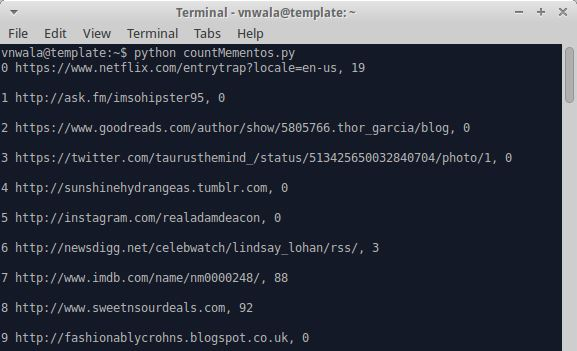
\includegraphics[width=3.0in]{countMementos}
    \caption{Screen Shot of countMementos.py at work}
    \label{fig:3}
\end{figure}
\begin{figure}
    \centering
    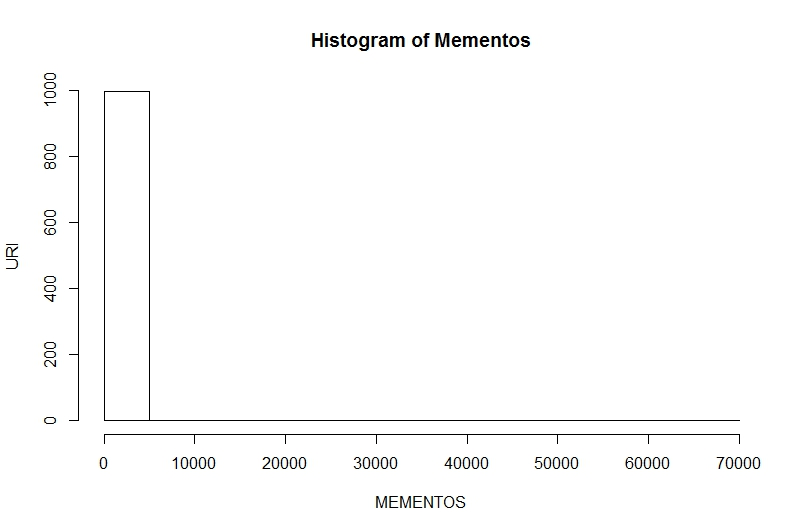
\includegraphics[width=3.0in]{histogram}
    \caption{Screen Shot of histogram From Rstudio}
    \label{fig:4}
\end{figure}
\begin{figure}
    \centering
    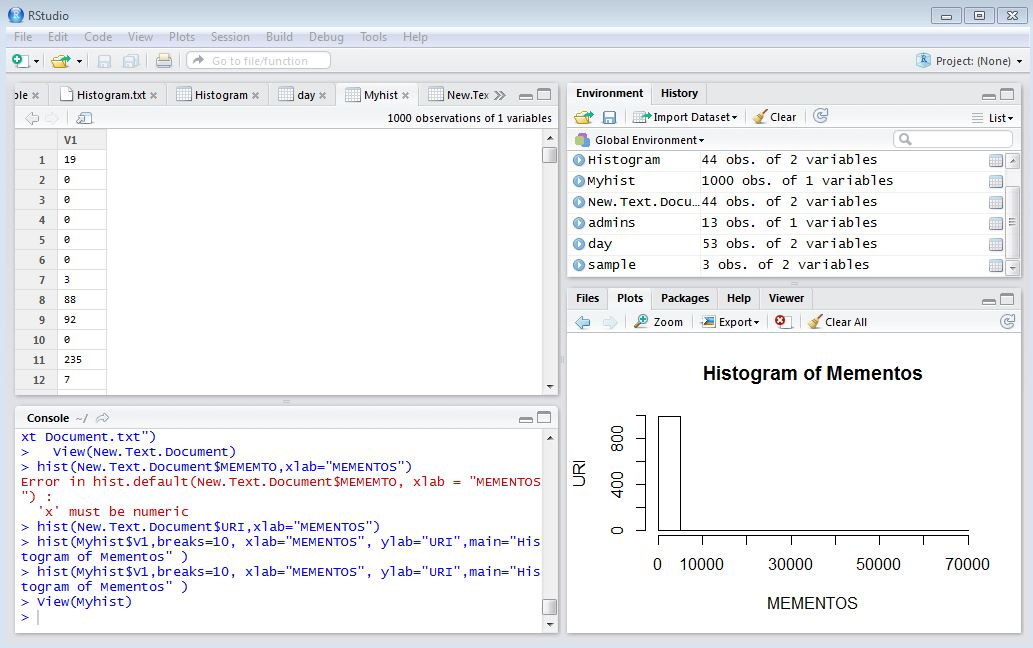
\includegraphics[width=5.0in]{RstudioLayout}
    \caption{Screen Shot of RstudioLayout}
    \label{fig:5}
\end{figure}

\end{homeworkProblem}
\clearpage

%----------------------------------------------------------------------------------------
%	PROBLEM 3
%----------------------------------------------------------------------------------------

\begin{homeworkProblem}


3.  Estimate the age of each of the 1000 URIs using the "Carbon Date" tool:

http://ws-dl.blogspot.com/2013/04/2013-04-19-carbon-dating-web.html

Note: you'll have better luck downloading and installing the tool 
rather than using the web service (which will run slowly and likely
be unreliable).

For URIs that have  greater than Zero Mementos and an estimated creation date,
create a graph with age (in days) on one axis and number of mementos
on the other.

%Listing \ref{local.py} shows a Python script to carbon URIs.
\lstinputlisting[breaklines=true, caption=CarbonDating URIs]{local.py}
I modified the code local.py given to use to perform this task, collecting only the variables I needed. I also wrote a script to convert the datetime variable to days so that I could construct my plot.

I had only 53 URIs with Memento greater than zero and also had Estimated creation date. Hence 53 points to plot a graph

\begin{figure}
    \centering
    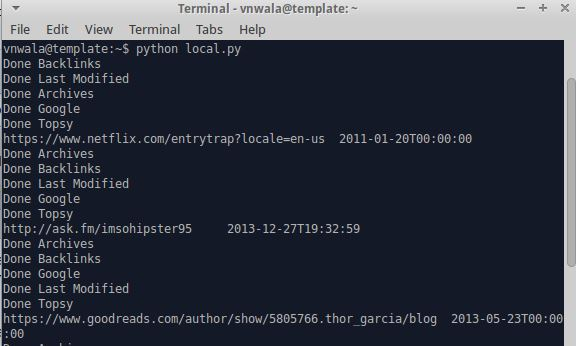
\includegraphics[width=5.0in]{local}
    \caption{Screen Shot of local.py at work}
    \label{fig:6}
\end{figure}
\clearpage
\begin{figure}
    \centering
    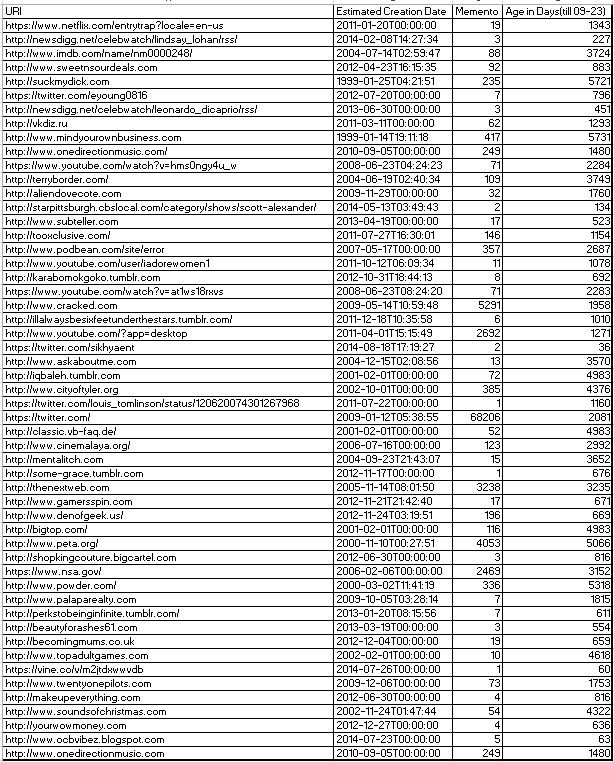
\includegraphics[width=5.0in]{Tablegraph}
    \caption{Screen Shot Mementos and age in Days}
    \label{fig:7}
\end{figure}

%Listing \ref{calculateAge.py} shows a Python script to calculte the Age of URIs .
\lstinputlisting[breaklines=true, caption=Python script to calculte the Age of URIs]{calculateAge.py}
\begin{figure}
    \centering
    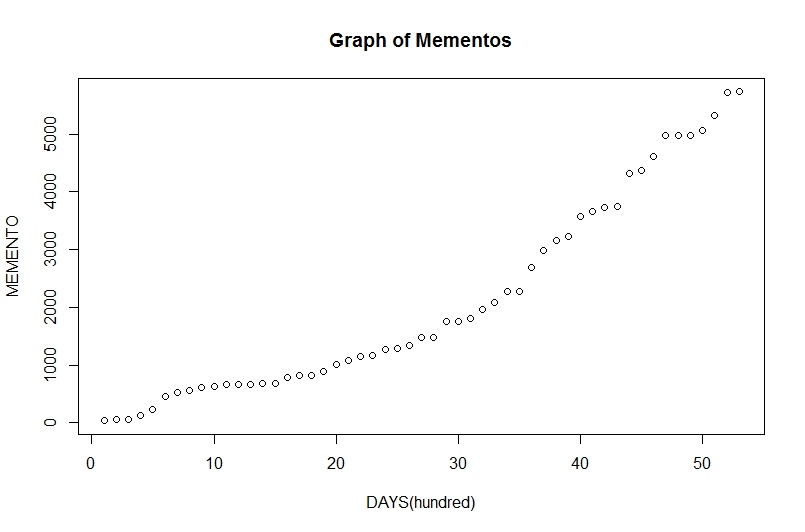
\includegraphics[width=5.0in]{graphPlot}
    \caption{Mementos Vs Age in Hundred Days}
    \label{fig:8}
\end{figure}
\clearpage
\begin{figure}
    \centering
    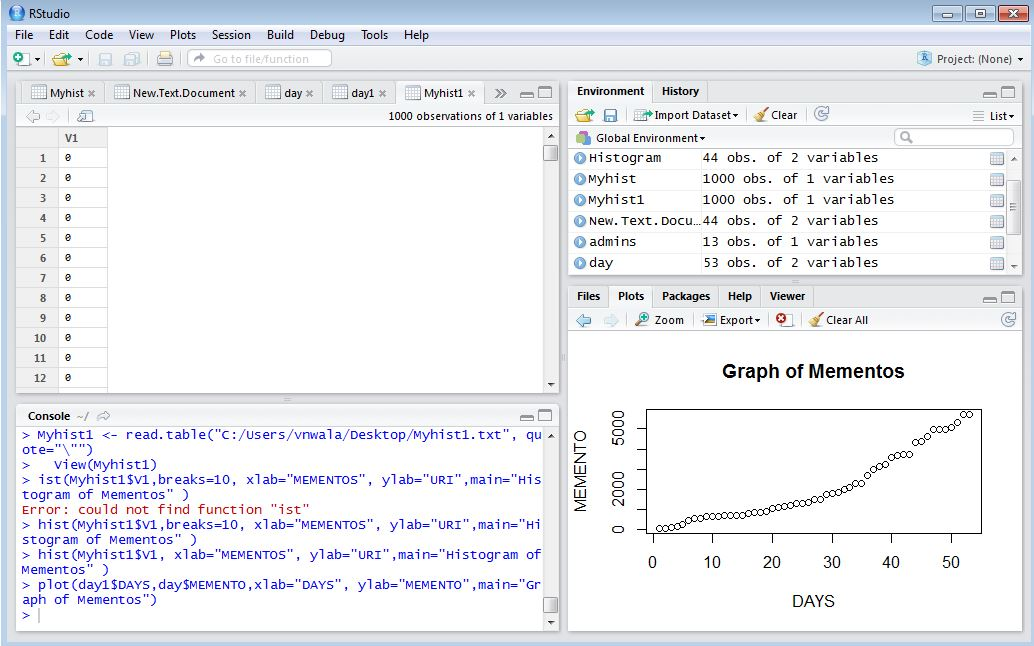
\includegraphics[width=5.0in]{RgraphLayout}
    \caption{Screen Shot of RgraphLayout}
    \label{fig:9}
\end{figure}
\end{homeworkProblem}

\clearpage

%----------------------------------------------------------------------------------------
%	OBSERVATIONS AND CONCLUSIONS
%----------------------------------------------------------------------------------------
\section{OBSERVATIONS AND CONCLUSIONS}
Firstly I will like to say that the URLs where randomly selected, some of which might be obscene sites or morally unworthy, there was no intent be offensive.

Secondly I noticed that my Histogram did not come out well because of the noisy data. I decided to remove all values of Mememto equal to zero and plot another histogram and a got the result above.

Thirdly I submitted only my final versions of text files, hence they might have  different filenames from that seen in my program code.

\begin{figure}
    \centering
    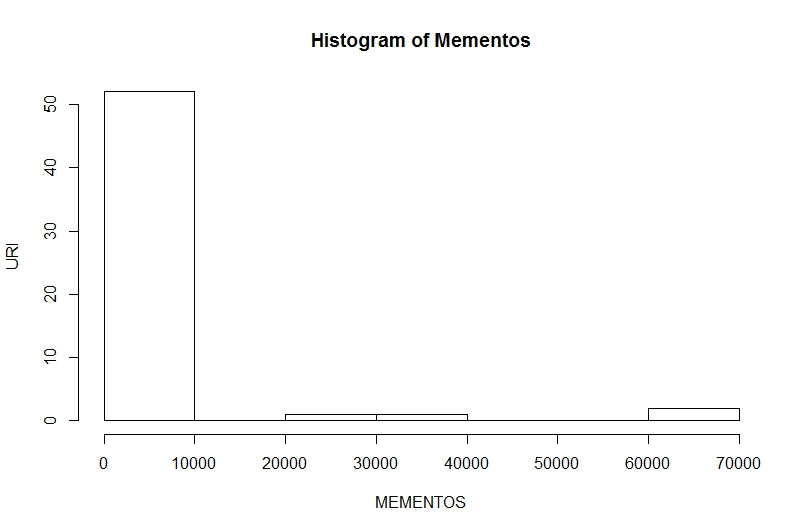
\includegraphics[width=5.0in]{Histogram_memento}
    \caption{Screen Shot of Histogram without Mementos equal to Zero}
    \label{fig:9}
\end{figure}



%----------------------------------------------------------------------------------------

\end{document}
